\documentclass[11pt,]{article}
\usepackage{mathpazo}
\usepackage{amssymb,amsmath}
\usepackage{ifxetex,ifluatex}
\usepackage{fixltx2e} % provides \textsubscript
\ifnum 0\ifxetex 1\fi\ifluatex 1\fi=0 % if pdftex
  \usepackage[T1]{fontenc}
  \usepackage[utf8]{inputenc}
\else % if luatex or xelatex
  \ifxetex
    \usepackage{mathspec}
    \usepackage{xltxtra,xunicode}
  \else
    \usepackage{fontspec}
  \fi
  \defaultfontfeatures{Mapping=tex-text,Scale=MatchLowercase}
  \newcommand{\euro}{€}
\fi
% use upquote if available, for straight quotes in verbatim environments
\IfFileExists{upquote.sty}{\usepackage{upquote}}{}
% use microtype if available
\IfFileExists{microtype.sty}{%
\usepackage{microtype}
\UseMicrotypeSet[protrusion]{basicmath} % disable protrusion for tt fonts
}{}
\usepackage{graphicx}
\makeatletter
\def\maxwidth{\ifdim\Gin@nat@width>\linewidth\linewidth\else\Gin@nat@width\fi}
\def\maxheight{\ifdim\Gin@nat@height>\textheight\textheight\else\Gin@nat@height\fi}
\makeatother
% Scale images if necessary, so that they will not overflow the page
% margins by default, and it is still possible to overwrite the defaults
% using explicit options in \includegraphics[width, height, ...]{}
\setkeys{Gin}{width=\maxwidth,height=\maxheight,keepaspectratio}
\ifxetex
  \usepackage[setpagesize=false, % page size defined by xetex
              unicode=false, % unicode breaks when used with xetex
              xetex]{hyperref}
\else
  \usepackage[unicode=true]{hyperref}
\fi
\hypersetup{breaklinks=true,
            bookmarks=true,
            pdfauthor={Matthew A. Barbour\^{}\{1,2,\textbackslash{}ast\}},
            pdftitle={Predicting the effects of character displacement on food-web dynamics},
            colorlinks=true,
            citecolor=blue,
            urlcolor=black,
            linkcolor=black,
            pdfborder={0 0 0}}
\urlstyle{same}  % don't use monospace font for urls
\setlength{\parindent}{0pt}
\setlength{\parskip}{6pt plus 2pt minus 1pt}
\setlength{\emergencystretch}{3em}  % prevent overfull lines
\setcounter{secnumdepth}{0}

%%% Use protect on footnotes to avoid problems with footnotes in titles
\let\rmarkdownfootnote\footnote%
\def\footnote{\protect\rmarkdownfootnote}


  \title{Predicting the effects of character displacement on food-web dynamics}
    \author{Matthew A. Barbour\(^{1,2,\ast}\)}
    \date{}
  
%%% From AmNat_MS_template.tex
%\documentclass[11pt]{article}
%\usepackage[sc]{mathpazo} %Like Palatino with extensive math support
\usepackage{fullpage}
%\usepackage[authoryear,sectionbib,sort]{natbib}
\linespread{1.7}
%\usepackage[utf8]{inputenc}
\usepackage{lineno}

%%%%%%% Sections not currently working properly
%\usepackage{titlesec}
%\titleformat{\section}[block]{\Large\bfseries\filcenter}{\thesection}{1em}{}
%\titleformat{\subsection}[block]{\Large\itshape\filcenter}{\thesubsection}{1em}{}
%\titleformat{\subsubsection}[block]{\large\itshape}{\thesubsubsection}{1em}{}
%\titleformat{\paragraph}[runin]{\itshape}{\theparagraph}{1em}{}[. ]\renewcommand{\refname}{Literature Cited}

%%% My added packages
%\usepackage{amsmath} % for matrices
%\usepackage{graphicx} % for organizing figures
%\usepackage{lmodern} % for tilde
%\usepackage[T1]{fontenc} % for tilde

%%%%%%%%% Previous - likely useful though
%\usepackage{setspace}\doublespacing
%\usepackage{float}
%\let\origfigure\figure
%\let\endorigfigure\endfigure
%\renewenvironment{figure}[1][2] {
%    \expandafter\origfigure\expandafter[H]
%} {
%    \endorigfigure
%}

\begin{document}

\maketitle


\noindent 1. University of British Columbia, Department of Zoology,
Vancouver, BC V6T 1Z4, Canada;

\noindent 2. University of Zurich, Department of Evolutionary Biology
and Environmental Studies, Winterthurerstrasse 190, 8057 Zurich,
Switzerland;

\(^\ast\) Corresponding author; e-mail:
\href{mailto:matthew.barbour@ieu.uzh.ch}{\nolinkurl{matthew.barbour@ieu.uzh.ch}}

\bigskip

\emph{Manuscript elements}: Figure 1, figure 2, figure 3, figure 4. All
figures should be printed in color.

\bigskip

\emph{Keywords}: competition; eco-evolutionary dynamics;
consumer-resource interactions; adaptive radiation; ecological community

\bigskip

\emph{Manuscript type}: Note.

\bigskip

\footnotesize Prepared using an \emph{Am. Nat.} inspired \LaTeX{}
template for Rmarkdown. \normalsize

\linenumbers{} \modulolinenumbers[3]

\newpage

\section{Abstract}\label{abstract}

\newpage

\section{Introduction}\label{introduction}

Ecological character displacement is thought to be a key evolutionary
process generating biodiversity (Dolph Schluter 2000; D. W. Pfennig and
Pfennig 2010; but see Stuart and Losos 2013). Ecological character
displacement describes the ``process of phenotypic evolution in a
species generated or maintained by {[}exploitative{]} resource
competition with one or more coexisting species'' (Dolph Schluter 2000).
Over the past 40 years, a large body of theoretical (e.g. Lawlor and
Smith 1976; P A Abrams 1986; Doebeli 1996; Taper and Chase 1985) and
empirical (reviewed in: Dolph Schluter 2000; Dayan and Simberloff 2005;
Stuart and Losos 2013) work has been generated to understand the
scenarios under which exploitative competition for resources leads to
the divergence of consumer foraging traits. The general result emerging
from these studies is that, if resources are nutritionally substitutable
(Peter A Abrams 1987; Fox and Vasseur 2008) and there is no other strong
source of density dependence acting on consumers (P A Abrams 1986), then
resource competition drives the divergence of consumer foraging traits
{[}Lawlor and Smith (1976); Taper and Chase (1985)). This process is not
simply driven by ecological differences, but creates an eco-evolutionary
feedback that drives further differentiation. This key insight was made
by theoretical models that explicitly included resource dynamics as a
mediator of competition in driving evolutionary change (Lawlor and Smith
1976; P A Abrams 1986; Taper and Chase 1985).

Although explicit models of resources gave key insights to the evolution
of character displacement, the ecological feedback onto
consumer-resource dynamics have received surprisingly little attention.
This is likely because character displacement has been primarily studied
through the lens of competition and coexistence theory {[}Lawlor1976;
Germain2018{]}. For example, early theoretical work by Lawlor and Smith
(1976) showed that ecological character displacement promotes
coexistence by favoring specialized consumers that experience reduced
interspecific competition. On the other hand, specialization often
increases a consumer's ability to capture a specific resource. A well
known consequence of increased foraging efficiency is resource
suppression, which if sufficient enough, can generate oscillations, and
hence less stable, consumer-resource dynamics {[}Rosenzweig 1971;
Murdoch et al. 2003; McCann 2011{]}. NEED A LAST SENTENCE TO WRAP IT UP,
HIGHLIGHTING HOW A FOOD-WEB PERSPECTIVE MAY YIELD NEW ECOLOGICAL
INSIGHTS AND GIVE A CONTRASTING PERSPECTIVE TO COEXISTENCE THEORY.
PERHAPS A I NEED TO INCLUDE A SENTENCE MID-WAY THROUGH SUGGESTING THAT A
FOOD-WEB PERSPECTIVE MAY GIVE QUALITATIVELY DIFFERENT INSIGHTS. IT MAY
BE NICE TO BRING IN THE SPATIAL COUPLING WORK OF MCCANN SUGGESTING THAT
SPECIALIZATION CAN COUPLE FOOD-WEBS, BUT THIS WAS ONLY WITH ONE TOP
PREDATOR (I.E. NO CONSUMERS\ldots{}LOOK AT OLD TEXT FOR WORDING
SUGGESTIONS.)

Here, I address this knowledge gap by building a mathematical model to
examine how ecological character displacement affects consumer-resource
dynamics in a food-web context. I address two questions: (1) How does
ecological character displacement affect resource abundances? (2) How
does character displacement affect food-web stability? To test the
generality of these ecological effects, I examined three different
foraging scenarios: (i) resources occur in the same habitat and
consumers exhibit a linear functional response (e.g. MacArthur (1972);
Lawlor and Smith (1976)); (ii) resources occur in different habitats and
consumers exhibit a linear functional response (e.g. Lawlor and Smith
(1976)); (iii) resources occur in distinct habitats and consumers
exhibit a more realistic functional response (K S McCann, Rasmussen, and
Umbanhowar 2005). I also explore the contingency of these effects to
different assumptions about evolutionary trade-offs in consumer foraging
traits. I focus on the ecological side of these dynamics because the
evolutionary aspects have been well characterized (Lawlor and Smith
1976; Taper and Chase 1985; P A Abrams 1986). I show that the
consequences of character displacement on food-web dynamics are not
always intuitive and depend on the foraging scenario and tradeoff in
consumer traits.

\section{Methods and Results}\label{methods-and-results}

\subsection{Underlying Food-web
Dynamics}\label{underlying-food-web-dynamics}

To examine how ecological character displacement affects
consumer-resource interactions and food-web dynamics, I analyzed a
continuous-time model of two consumers (\(C_1,C_2\)) competing for two
shared resources (\(R_1,R_2\)):

\[\frac{dR_1}{dt}=r_1K_1(1-\frac{R_1}{K_1})-F_{11}(R_1)C_1-F_{21}(R_1)C_2,\]
\[\frac{dR_2}{dt}=r_2K_2(1-\frac{R_2}{K_2})-F_{12}(R_2)C_1-F_{22}(R_2)C_2,\]
\[\frac{dC_1}{dt}=e_{11}F_{11}(R_1)C_1+e_{12}F_{12}(R_2)C_1-m_1C_1,\]
\[\frac{dC_2}{dt}=e_{21}F_{21}(R_1)C_2+e_{22}F_{22}(R_2)C_2-m_2C_2,\]

where \(r_i\) represents the intrinsic growth rate of resource \(i\),
\(K_i\) represents the carrying capacity of resource \(i\), \(e_{ji}\)
represents the conversion efficiency of resource \(i\) into consumer
\(j\), and \(m_j\) represents the mortality rate of consumer \(j\).
\(F_{ji}(R_i)\) represents consumer \(j\)'s feeding rate
(i.e.~functional response) on resource \(i\). This model is a useful
characterization of a scenario where consumers compete for two distinct
resources (e.g.~zooplankton and benthic invertebrates) rather than if
resources are better characterized by a continuous trait distribution
(e.g.~seed size, see Taper and Chase (1985) for an example). In the
scenario where consumer feeding rates increase linearly with resource
density, such that \(F_{ji}(R_i)=a_{ji}R_i\) where \(a_{ji}\) is the
attack rate of consumer \(j\) on resource \(i\), then this model becomes
MacArthur's model of resource competition (MacArthur (1972)). The
evolution of consumer attack rates in this model (and several
extensions) have been analyzed in detail (Lawlor and Smith (1976); P A
Abrams (1986)), with the general result being divergent character
displacement. I say consumers have undergone divergent character
displacement if there evolved attack rates are more specialized, defined
as \(|\frac{a_{ii}}{a_{ii}+a_{ij}}-0.5|\), when evolving with a
competing consumer. I focus here on the ecological consequences of this
adaptive divergence.

To investigate the ecological consequences, I studied the effect of
adaptive divergence in consumers on resource densities and the stability
of the entire food web at equilibrium. An equilibrium is reached when
the four rates of change in the above equations are 0, and solving the
system at this point gives equilibrium densities for each resource
(\(\hat R_1,\hat R_2\)) and consumer (\(\hat C_1,\hat C_2\)). At the
coexistence equilibrium (i.e., where
\(\hat R_1,\hat R_2, \hat C_1,\hat C_2 > 0\)), I calculated resource
densities and performed a linear stability analysis (Otto and Day 2007).
This stability analysis derives the dominant (largest in absolute value)
eigenvalue, \(\lambda\), which determines whether (and how readily) the
food web, when perturbed a small amount, will return to equilibrium (see
supplementary material for derivation). Together, these two measures
indicate how ecological character displacement affects resource
densities and food-web stability.

I examine the effects of this inevitable divergence in attack rates on
food-web dynamics by (i) deriving analytical expressions for the
relationship between attack rates and food-web dynamics and (ii)
simulating the effects of competition on the eco-evolutionary dynamics
of consumers and resources. To gain analytical insight, I assume that
resources are equivalent (\(r=r_1=r_2\) and \(K=K_1=K_2\)) as well as
consumers (\(e=e_{11}=e_{12}=e_{21}=e_{22}\); \(m=m_1=m_2\)), except
that consumer attack rates are mirror images of each other
(\(a_{ii}=a_{11}=a_{22}\); \(a_{ij}=a_{12}=a_{21}\)). While this
scenario is arguably simplistic, it allows me to isolate the effects of
ecological character displacement.

To simulate eco-evolutionary dynamics, I used an Adaptive Dynamics
approach. At each evolutionary time step, I created a mutant consumer by
randomly choosing a consumer and modifying its attack rate on one
resource by either subtracting or adding a small constant (0.001 in the
following simulations) with equal probability. The mutant's attack rate
on the other resource was determined by a tradeoff, such that
\(\big(a_{ii}/{A}\big)^n+\big(a_{ij}/{A}\big)^n=1\), where \(A\) is the
total investment in attack rates and \(n\) describes the shape of the
tradeoff (Sargent and Otto 2006). This function has the useful property
that it differentiates between cases where intermediate combinations of
\(a_{ii}\) and \(a_{ij}\) are higher, on average, than the extremes
(when \(n>1\), green line in Fig. \ref{fig:Tradeoff}) or, conversely,
where the two extremes are higher, on average, than intermediate
investments (when \(n<1\), orange line Fig. \ref{fig:Tradeoff}). When
\(n=1\), the tradeoff function is linear, and all combinations of
\(a_{ii}\) and \(a_{ij}\) have the same total attack rate (blue line in
Fig. \ref{fig:Tradeoff}). Assuming the mutant consumer was rare, I then
determined whether the mutant had higher relative fitness than the
resident consumer, and thus could invade and replace the resident
consumer. If the mutant was able to invade, I updated the attack rate of
the resident consumer to the mutant attack rate and allowed consumer and
resource dynamics to reach a steady state. I then repeated the
simulation up to 10,000 times, which was sufficient for consumers to
either reach an evolutionary stable strategy (ESS, Smith and Price 1973)
or an evolutionary limit (e.g. \(\frac{a_{ii}}{a_{ii}+a_{ij}}\) is
constrained to a maximum of 1 and minimum of 0).

\begin{figure}
\centering
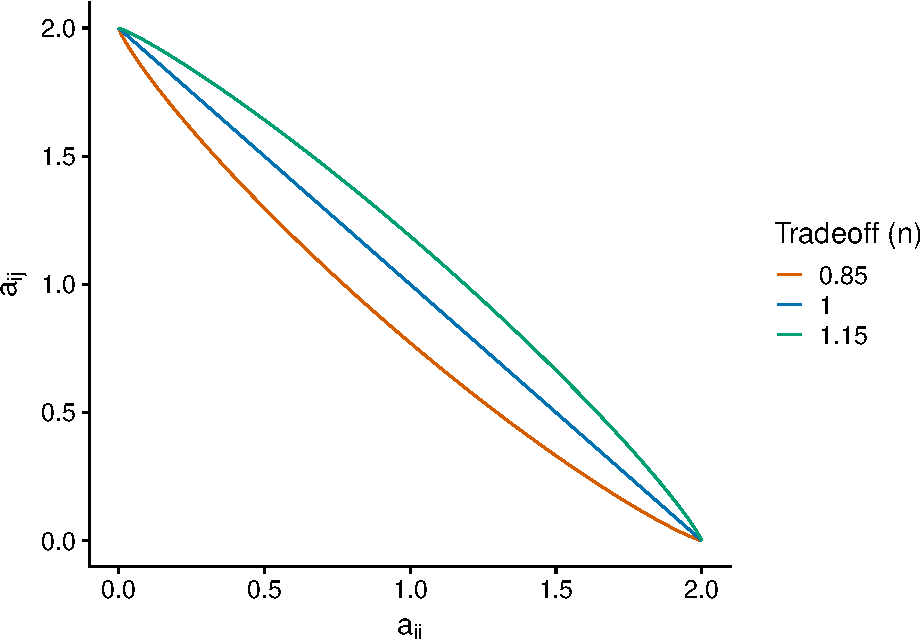
\includegraphics{manuscript_ECD_model_files/figure-latex/Tradeoff-1.pdf}
\caption{\label{fig:Tradeoff}Tradeoff forms for consumer attack rates.}
\end{figure}

\subsection{Consumers Forage For Both Resources
Simultaneously}\label{consumers-forage-for-both-resources-simultaneously}

When both consumers and resources are present, the density of resources
at equilibrium are equivalent (\(\hat R = \hat R_1 = \hat R_2\)) and are
determined by the following equation (derivation in supplementary
material):

\[\hat{R}=\frac{1}{a_{ii}+a_{ij}}\cdot\frac{m}{e}\] A key determinant of
resource density in this model is the consumer's total attack rate,
\(a_{ii}+a_{ij}\). Therefore, the ecological consequences of character
displacement depend on how the tradeoff influences the evolution of
consumer attack rates.

My simulations show that the shape of the attack-rate tradeoff
qualitatively affects the relationship between character displacement
and resource density (Fig. \ref{fig:MacArthur_Resources}). For example,
if consumer's are constrained by a linear tradeoff (blue lines), then
there is no net change in total attack rate (Fig.
\ref{fig:MacArthur_Resources}A) and character displacement has no effect
on resource densities (Fig. \ref{fig:MacArthur_Resources}B). If the
tradeoff is concave down (green lines), then resource abundances can
actually increase under character displacement (Fig.
\ref{fig:MacArthur_Resources}B). This is because the total attack rate
of consumers is maximized at intermediate values (\(a_{ii}=a_{ij}\)) and
decreases as consumers diverge (Fig. \ref{fig:MacArthur_Resources}A).
When the tradeoff is concave up (orange lines), character displacement
suppresses resource densities due to the increase in total attack rates
(Fig. \ref{fig:MacArthur_Resources}A,B). Although the equation I derived
for resource density was for the scenario where both consumers and both
resources are present, it accurately predicts the density of resources
when a single consumer reaches its ESS (triangles on respective colored
lines in Fig. \ref{fig:MacArthur_Resources}B). This is because a single
consumer evolves to be a generalist that has equal attack rates on each
resource (triangles at 0.5 along x-axis in Fig.
\ref{fig:MacArthur_Resources}A), resulting in equivalent resource
densities.

The effect of character displacement on resource density closely matches
its impact on food-web stability (Fig. \ref{fig:Stability}). For
example, when character displacement results in resource suppression
(orange), there is a corresponding decrease in stability. Similarly, if
character displacement does not influence resource densities (blue),
then there is no corresponding effect on stability. Curiously, this
match between impact on resources and stability breakdowns with the
concave down tradeoff (green).

\begin{figure}
\centering
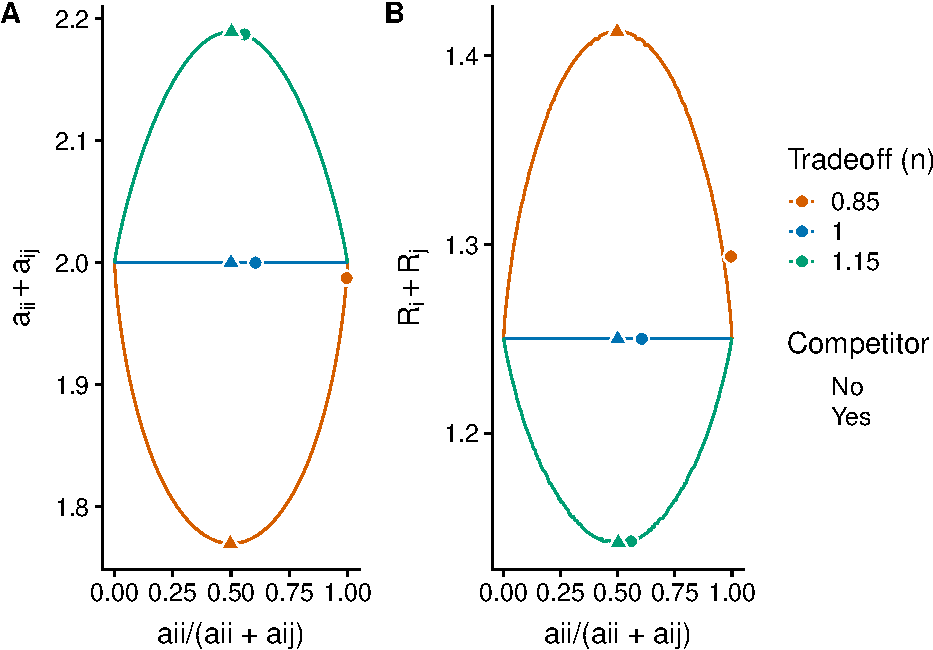
\includegraphics{manuscript_ECD_model_files/figure-latex/MacArthur_Resources-1.pdf}
\caption{\label{fig:MacArthur_Resources}Effect of character displacement
on total attack rates (A) and resource densities (B) when consumers can
forage for both resources simultaneously.}
\end{figure}

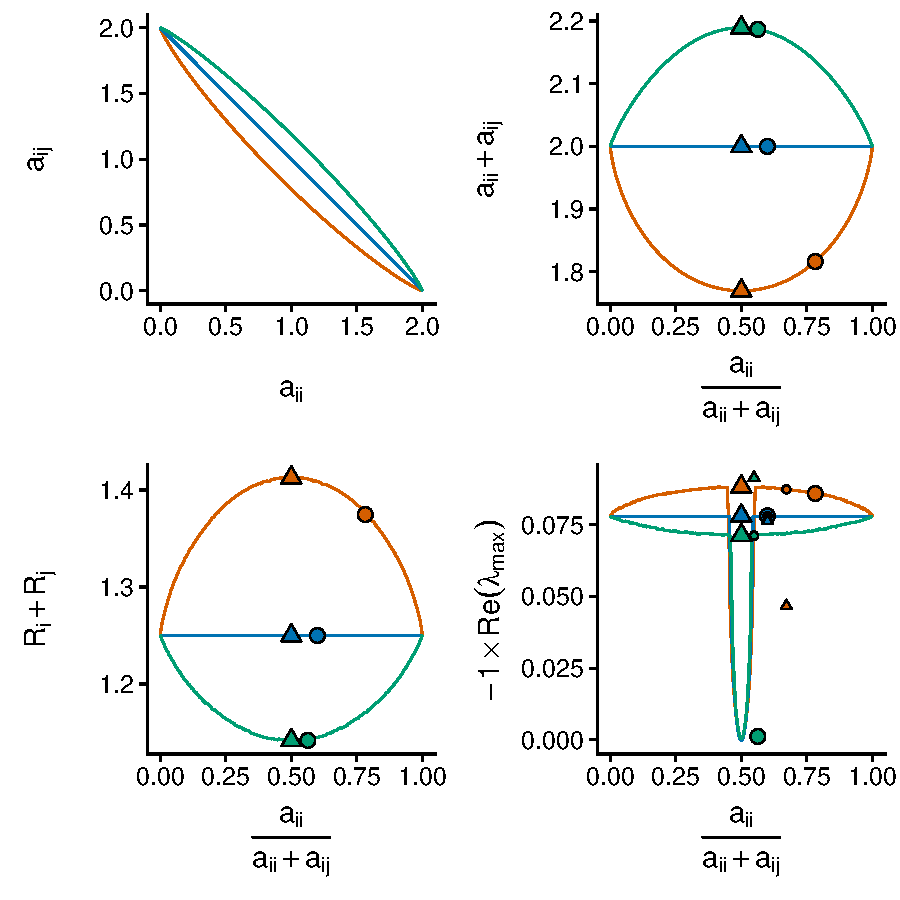
\includegraphics{Figure_ECD_MacArthur.pdf}

\subsection{\texorpdfstring{Consumers \emph{cannot} forage for both
resources
simulanteously}{Consumers cannot forage for both resources simulanteously}}\label{consumers-cannot-forage-for-both-resources-simulanteously}

The only character displacement model that I am aware of that modeled
resources in different habitats was one examined by Lawlor and Smith
(1976). This model takes the same form as the previous model, except now
the consumer's feeding rate takes the form:

\[F_{ji}(R_i)=w_{ji}a_{ji}R_i\]

where \(w_{ji}\) represents the proportion of time consumer \(j\) spends
foraging in a habitat where only resource \(j\) is found (i.e.~habitat
preference). Note that since \(w_{ji}\) is a proportion that
\(w_{jj}=1-w_{ji}\). As with attack rates, I assume that consumer
habitat preferences are mirror images of each other
(\(w=w_{11}=w_{22}\)). In Lawlor and Smith (1976)'s detailed
evolutionary analysis of this model, they again always observe divergent
character displacement.

To examine the ecological consequences of this model, I again derive the
equilibrium solution when both consumers and both resources are present.
Again, resource densities are equivalent at this equilibrium
(\(\hat R = \hat R_1 = \hat R_2\) when both consumers and resources
present), but are now determined by the following equation (derivation
in supplementary material):

\[\hat{R}=\frac{1}{wa_{ii}+(1-w)a_{ij}}\cdot\frac{m}{e}\]

This equation implies that if consumers evolve to become specialists on
resources that occur in their preferred habitat (e.g. \(w>0.5\) and
\(a_{ii}>a_{ij}\)), then the effective attack rate of consumers
(\(wa_{ii}+(1-w)a_{ij}\)) will always increase, regardless of the
tradeoff (Fig. \ref{fig:LS_Resources}A). Thus, character displacement
always results in resource suppression if consumers are competing for
resources that occur in different habitats (Fig.
\ref{fig:LS_Resources}B). Note that the shape of the tradeoff can modify
the effect of character displacement. This is not so much due to the
tradeoff affecting the magnitude of displacement (it does, but the
effect is minor), but because the form of the tradeoff affects resource
abundances when a single consumer has reached its ESS (triangles in Fig.
\ref{fig:LS_Resources}B). In contrast, resource densities reach a
similar value when consumers evolve in the presence of a competitor
(circles in Fig. \ref{fig:LS_Resources}B), because character
displacement tends to reach a constraint of complete specialization. It
is worth noting that in this foraging scenario, resource densities are
consistently higher at the single consumer ESS compared to the
predictions I derived for when both consumers are present (deviation of
triangles from respective colored lines in Fig.
\ref{fig:LS_Resources}B). This is likely because consumers actually
evolve to be slightly specialized on the resources that occur in their
non-preferred habitat (deviation of triangles from 0.5 along x-axis in
Fig. \ref{fig:LS_Resources}B).

The effect of character displacement on resource densities qualitatively
matches its negative effect of food-web stability (Fig.
\ref{fig:Stability}). This is not simply a consequence of having an
additional consumer in the system, but emerges from the eco-evolutionary
feedback between character displacement and resource suppression
(compare initial (small points) with evolved strategies (large points),
Fig. \ref{fig:Stability}). For example, when the tradeoff is concave up
(orange), then the four-species (small circle) food web actually starts
off as less stable than the three-species one (small triangle), but the
eco-evolutionary dynamics cause a switch in the pattern once they reach
their evolutionary stable strategies (large points).

\begin{figure}
\centering
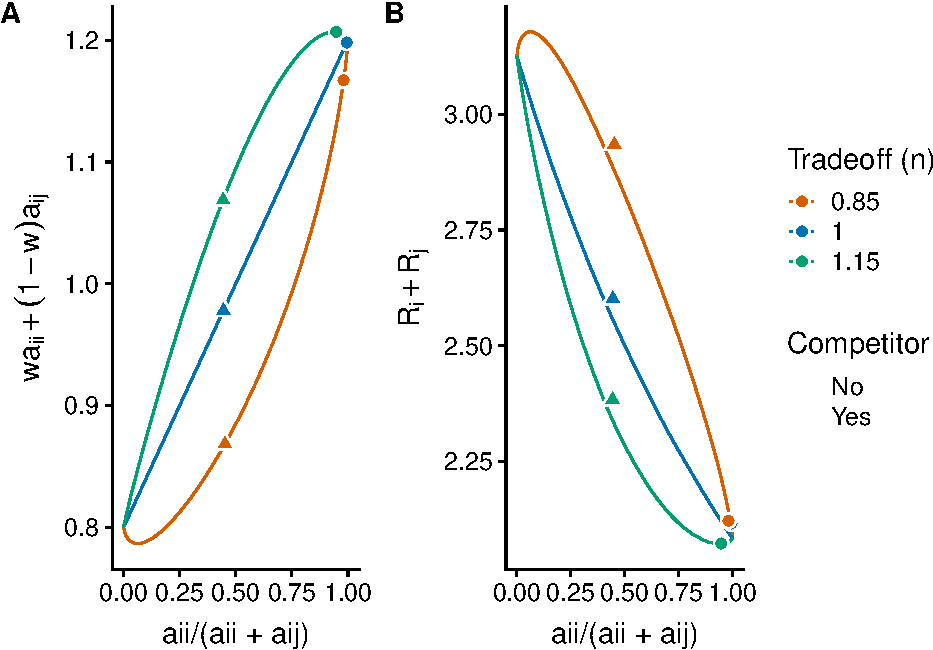
\includegraphics{manuscript_ECD_model_files/figure-latex/LS_Resources-1.pdf}
\caption{\label{fig:LS_Resources}Effect of character displacement on
effective attack rates (A) and resource densities (B) when consumers
cannot forage for resources simultaneously.}
\end{figure}

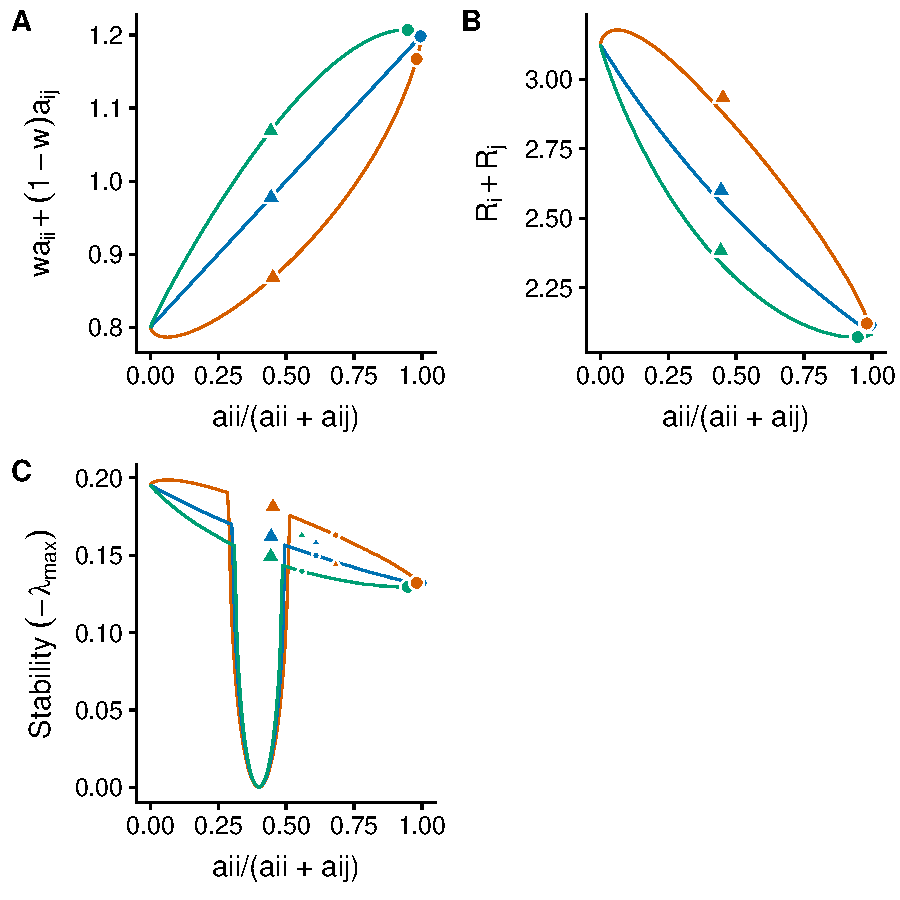
\includegraphics{Figure_ECD_LS.pdf}

\subsection{Adding A More Realistic Functional
Response}\label{adding-a-more-realistic-functional-response}

Thus far I have consider a simple type I functional response of
consumers foraging for resources in either the same or distinct
habitats.\\
For example, even if I consider a more realistic consumer functional
response (derived by K S McCann, Rasmussen, and Umbanhowar (2005)):

\[F_{ii}(R_i,R_j)=\frac{a_{ii}W_{ii}R_i}{1+a_{ii}hW_{ii}R_i+a_{ij}hW_{ij}R_j}\]

where consumer feeding rates on resource \(i\) are influenced by both
resource densities; saturate as resource densities increase (due to
handling time \(h\)); and consumer habitat preferences are modified by
relative resource densities, such that:

\[W_{ii}=\frac{wR_i}{wR_i+(1-w)R_j}\]

I still observe the same qualitative relationship between character
displacement and resource suppression (Fig. \ref{fig:McCann_Resources}
in Appendix). This is because resource competition always leads to
character divergence and equilibrium resource densities are governed by
similar dynamics (\emph{Mathematica} file with derivations available
upon request):

\[\hat{R}=\frac{1}{wa_{ii}+(1-w)a_{ij}}\cdot\frac{m}{e-hm}\]

I conducted the previous simulations on a scenario where the food web
remains locally stable (\(\operatorname{Re}(\lambda_{max})<0\)). Is it
possible that character displacement would ever result in a locally
unstable food web? To gain analytical insight to this question, I
examined the conditions governing the local stability of the
four-species food web when consumers exhibit a more realistic functional
response (K S McCann, Rasmussen, and Umbanhowar (2005)). I show that the
four-species food web will transition from having a locally stable
equilibrium to a limit cycle under the following conditions
(\emph{Mathematica} file with derivation available upon request):

\[wa_{ii}+(1-w)a_{ij} > \frac{e+hm}{hK(e-hm)}\]

Previously, I showed that character displacement always increases the
effective attack rate of consumers (\(wa_{ii}+(1-w)a_{ij}\)), regardless
of the the shape of the tradeoff (Fig. \ref{fig:LS_Resources}A). Thus,
character displacement is capable of pushing food webs to a point where
they are locally unstable. (it simple depends on the choice of
parameter, I could put a situation where evolution pushes it toward
local instability, or even the hopf bifurcation.)

\section{Discussion}\label{discussion}

I find that the foraging scenario qualitatively affects the relationship
between character displacement and resource densities.

Most models of character displacement have assumed a scenario where
consumers can forage for both resources simultaneously (e.g. Taper and
Chase 1985; P A Abrams 1986). This assumption may be valid for some
foraging scenarios (e.g.~Darwin's finches foraging for seeds); however,
in many situations consumers forage for resources that occur in
different habitats, and thus cannot forage for both simultaneously (K S
McCann, Rasmussen, and Umbanhowar 2005).

The effect of the foraging scenario on the relationship between
character displacement and resource densities appears to be quite
general.

Note that detecting this effect in nature would likely be difficult,
since a concave-down tradeoff results in relatively small displacement
relative to other tradeoff shapes (Lawlor and Smith (1976); green points
in Fig. \ref{fig:MacArthur_Resources}A,B).

Previous work has shown that consumers undergo divergent character
displacement regardless of the shape of the tradeoff (Lawlor and Smith
(1976); P A Abrams (1986)).

Important point: Criteria 5 in D Schluter and McPhail (1992) does not
make sense since character displacement usually alters resource
distributions. Think about this more.

Lawlor and Smith (1976) found that consumers still underwent divergent
character displacement regardless of whether consumers could or could
not forage for resources simultaneously.

These results do lead to an interesting prediction that could be tested
either experimentally or with field data. If consumers are competing for
resources that occur in different habitats, then greater character
displacement corresponds to a greater decrease in resource densities
(line trajectories in Fig. \ref{fig:LS_Resources}B). This prediction
likely only applies to comparisons within species where there is likely
little difference in the shape of the tradeoff among populations.

In general, I find that resource supression goes hand-in-hand with local
stability, a tendency that has been noted by others (Murdoch, Briggs,
and Nisbet (2003); Kevin S McCann (2011)).

The scenario where the relationship between character displacement and
resource suppression is the strongest is when the tradeoff in attack
rates is concave-up and consumers are competing for resources that occur
in different habitats (orange points in Fig. \ref{fig:LS_Resources}B and
Fig. \ref{fig:McCann_Resources}B). Prior work in threespine stickleback
suggests that the evolution of stickleback attack rates are constrained
by a concave-up tradeoff (Dolph Schluter (1993); Arnegard et al. (2014))
and that stickleback ecotypes are competing for resources that occur in
different habitats (benthic vs.~limnetic, D Schluter and McPhail
(1992)). Thus, I predict that ecological character displacement in
sticklebacks would suppress resource densities and decrease local
stability.

While measuring resource densities is relatively straightforward,
measuring stability is notoriously difficult. One of the more easy to
acquire empirical metrics of stability is the coefficient of variation
(\(CV=\frac{\sigma}{\mu}\)) as this only requires measurements of
resource (or consumer) densities over time. Interestingly, there is a
close correspondence between the coefficient of variation and the local
stability of a food web (Gellner, McCann, and Hastings (2016)). Thus, I
predict that character displacement in threespine stickleback will
increase the \(CV\) of resource (or consumer) densities.

Consumer and resource densities in these dynamical models can be
interpreted from either a population or biomass perspective (Yodzis and
Innes (1992); Murdoch, Briggs, and Nisbet (2003); Kevin S McCann
(2011)). For the stickleback system, you have data on seasonal dynamics
of resources in terms of both abundances and biomass. Within a season, I
do not expect stickleback abundances to be coupled to the abundances of
zooplankton and benthic invertebrates, given that stickleback reproduce
annually whereas zooplankton and benthic invertebrates can reproduce
many times within a season. Instead, I expect that stickleback biomass
will be coupled to the biomass of zooplankton and benthic invertebrates
within a season. This is because there will be lots of young stickleback
at the beginning of the season, and they will eat a lot of resources and
grow in size as the season progresses. If this is true, I also expect to
see the largest negative effect of stickleback on resource densities
late in the season.

Although I used an Adaptive Dynamics approach here, I expect that these
theoretical predictions would apply to models that assumed a different
genetic architecture of attack rates (e.g.~quantitative genetics). I
expect this because, time and time again, models that explicitly include
resource dynamics inevitably show that resource competition results in
divergent character displacement, regardless of the genetic architecture
of traits (see synthesis by Taper and Chase (1985)). Finally, my
conclusions only apply to biological resources that are nutritionally
substitutable. It would be interesting to extend these current analyses
to non-substitutable resources where convergent character displacement
is expected (Peter A Abrams (1987); Fox and Vasseur (2008)).

\section{Acknowledgements}\label{acknowledgements}

The content of this paper was greatly enhanced by numerous conversations
with Seth Rudman. Sally Otto provided much help in early analyses of the
mathematical model and I would not have been able to take the theory as
far as I did without her guidance and her pushing me.

Thank Ben Gilbert for his comment during a discussion of the model that
pushed me to take a comparative approach that looked across different
model structures to examine the generality of these results.

\section{References}\label{references}

\hypertarget{refs}{}
\hypertarget{ref-Abrams1986}{}
Abrams, P A. 1986. ``Character Displacement and Niche Shift Analyzed
Using Consumer-Resource Models of Competition.'' \emph{Theor. Popul.
Biol.} 29 (1): 107--60.

\hypertarget{ref-Abrams1987}{}
Abrams, Peter A. 1987. ``Alternative Models of Character Displacement
and Niche Shift. I. Adaptive Shifts in Resource Use When There Is
Competition for Nutritionally Nonsubstitutable Resources.''
\emph{Evolution} 41 (3). Wiley Online Library: 651--61.

\hypertarget{ref-Arnegard2014}{}
Arnegard, Matthew E, Matthew D McGee, Blake Matthews, Kerry B Marchinko,
Gina L Conte, Sahriar Kabir, Nicole Bedford, et al. 2014. ``Genetics of
Ecological Divergence During Speciation.'' \emph{Nature} 511 (7509):
307--11.

\hypertarget{ref-Dayan2005}{}
Dayan, Tamar, and Daniel Simberloff. 2005. ``Ecological and
Community-Wide Character Displacement: The Next Generation.''
\emph{Ecol. Lett.} 8 (8). Blackwell Science Ltd: 875--94.

\hypertarget{ref-Doebeli1996}{}
Doebeli, Michael. 1996. ``An Explicit Genetic Model for Ecological
Character Displacement.'' \emph{Ecology} 77 (2). Ecological Society of
America: 510--20.

\hypertarget{ref-Fox2008}{}
Fox, Jeremy W, and David A Vasseur. 2008. ``Character Convergence Under
Competition for Nutritionally Essential Resources.'' \emph{The American
Naturalist} 172 (5). The University of Chicago Press: 667--80.

\hypertarget{ref-Gellner2016}{}
Gellner, Gabriel, Kevin S McCann, and Alan Hastings. 2016. ``The Duality
of Stability: Towards a Stochastic Theory of Species Interactions.''
\emph{Theor. Ecol.} 9 (4): 477--85.

\hypertarget{ref-Lawlor1976}{}
Lawlor, Lawrence R, and J Maynard Smith. 1976. ``The Coevolution and
Stability of Competing Species.'' \emph{Am. Nat.} 110 (971).
{[}University of Chicago Press, American Society of Naturalists{]}:
79--99.

\hypertarget{ref-MacArthur1972}{}
MacArthur, R H. 1972. \emph{Geographical Ecology: Patterns in the
Distribution of Species}. Biology / {[}Princeton University Press{]}.
Princeton University Press.

\hypertarget{ref-McCann2005}{}
McCann, K S, J B Rasmussen, and J Umbanhowar. 2005. ``The Dynamics of
Spatially Coupled Food Webs.'' \emph{Ecol. Lett.} 8 (5). Blackwell
Science Ltd: 513--23.

\hypertarget{ref-McCann2011}{}
McCann, Kevin S. 2011. \emph{Food Webs (Mpb-50)}. Princeton University
Press.

\hypertarget{ref-Murdoch2003}{}
Murdoch, W W, C J Briggs, and R M Nisbet. 2003. \emph{Consumer-Resource
Dynamics}. Monographs in Population Biology. Princeton University Press.

\hypertarget{ref-Otto2007}{}
Otto, Sarah P, and Troy Day. 2007. \emph{A Biologist's Guide to
Mathematical Modeling in Ecology and Evolution}. Princeton University
Press.

\hypertarget{ref-Pfennig2010}{}
Pfennig, David W, and Karin S Pfennig. 2010. ``Character Displacement
and the Origins of Diversity.'' \emph{Am. Nat.} 176 Suppl 1 (December):
S26--44.

\hypertarget{ref-Sargent2006}{}
Sargent, Risa D, and Sarah P Otto. 2006. ``The Role of Local Species
Abundance in the Evolution of Pollinator Attraction in Flowering
Plants.'' \emph{Am. Nat.} 167 (1): 67--80.

\hypertarget{ref-Schluter1992}{}
Schluter, D, and J D McPhail. 1992. ``Ecological Character Displacement
and Speciation in Sticklebacks.'' \emph{Am. Nat.} 140 (1): 85--108.

\hypertarget{ref-Schluter1993}{}
Schluter, Dolph. 1993. ``Adaptive Radiation in Sticklebacks: Size,
Shape, and Habitat Use Efficiency.'' \emph{Ecology} 74 (3): 699--709.

\hypertarget{ref-Schluter2000}{}
---------. 2000. ``Ecological Character Displacement in Adaptive
Radiation.'' \emph{Am. Nat.} 156 (S4): S4--S16.

\hypertarget{ref-Smith1973}{}
Smith, J Maynard, and G R Price. 1973. ``The Logic of Animal Conflict.''
\emph{Nature} 246 (November). Nature Publishing Group: 15.

\hypertarget{ref-Stuart2013}{}
Stuart, Yoel E, and Jonathan B Losos. 2013. ``Ecological Character
Displacement: Glass Half Full or Half Empty?'' \emph{Trends Ecol. Evol.}
28 (7): 402--8.

\hypertarget{ref-Taper1985}{}
Taper, Mark L, and Ted J Chase. 1985. ``Quantitative Genetic Models for
the Coevolution of Character Displacement.'' \emph{Ecology} 66 (2).
Ecological Society of America: 355--71.

\hypertarget{ref-Yodzis1992}{}
Yodzis, P, and S Innes. 1992. ``Body Size and Consumer-Resource
Dynamics.'' \emph{Am. Nat.} 139 (6). {[}University of Chicago Press,
American Society of Naturalists{]}: 1151--75.

\newpage

\section{Appendix: More realistic functional
response}\label{appendix-more-realistic-functional-response}

\begin{figure}
\centering
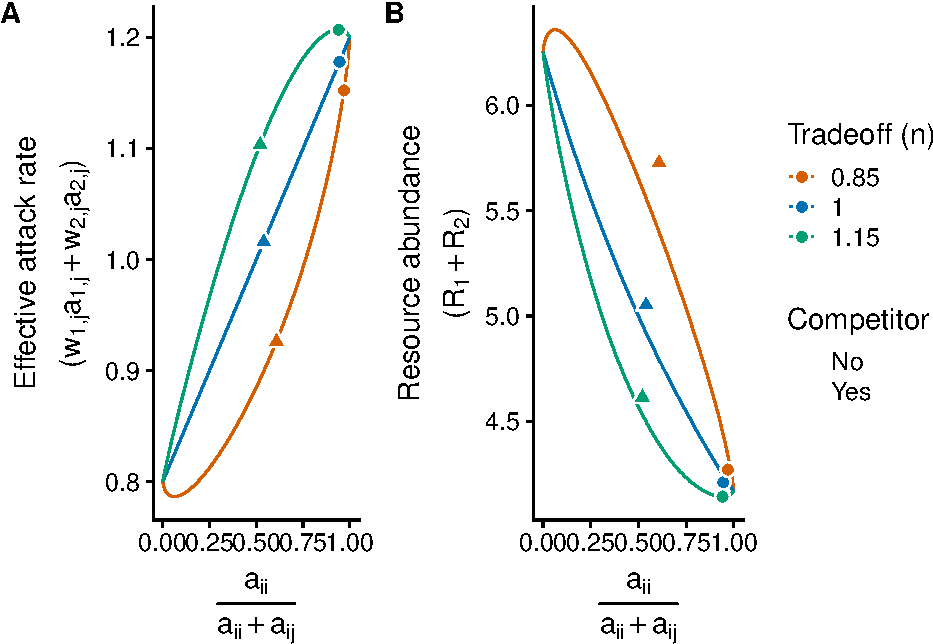
\includegraphics{manuscript_ECD_model_files/figure-latex/McCann_Resources-1.pdf}
\caption{\label{fig:McCann_Resources}Effect of character displacement on
total attack rates (A) and resource densities (B) when consumers exhibit
a more realistic functional response.}
\end{figure}

\begin{figure}
\centering
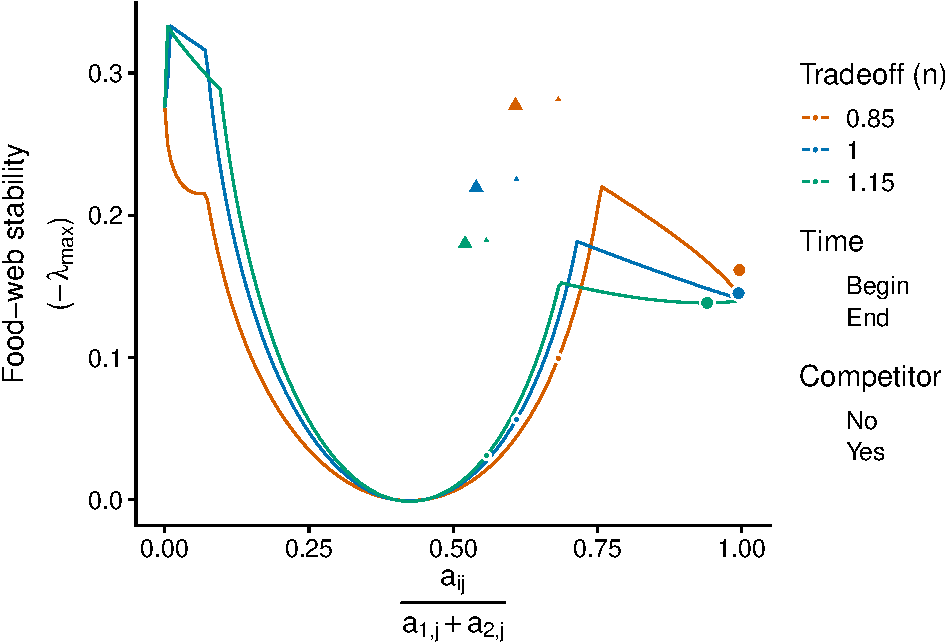
\includegraphics{manuscript_ECD_model_files/figure-latex/Stability_McCann-1.pdf}
\caption{\label{fig:Stability_McCann}Effect of character displacement on
local stability when consumers exhibit a more realistic functional
response.}
\end{figure}

\end{document}
